\chapter{Estado del Arte}\label{chapter:state-of-the-art}

En el presente capítulo se exponen los conceptos básicos que permiten familiarizarse con el funcionamiento de las \textit{blockchains} y con las funciones y componentes específicos de Hyperledger Fabric. Además, se analizarán las bibliotecas que  actualmente posibilitan el desarrollo de contratos inteligentes en otros lenguajes de programación (Go, Java, Node.js).

\section{Qué es una Blockchain}
En esencia, una blockchain es un \textbf{\textit{ledger}} distribuido que registra todas las transacciones que tienen lugar en la red. El \textit{ledger} de una \textit{blockchain} a menudo se describe como descentralizado porque se replica entre muchos participantes de la red, cada uno de los cuales colabora en su mantenimiento.

La información registrada en una \textit{blockchain}, además de ser \textbf{descentralizada} y \textbf{colaborativa}, sólo se puede agregar. Esto significa que no se puede modificar los datos de una transacción después de ser añadida al \textit{ledger}. Esta propiedad de inmutabilidad simplifica la determinación de la procedencia de la información pues los participantes pueden estar seguros de que esta no ha cambiado después de añadirse a la \textit{blockchain}.

Con el fin de respaldar la actualización constante de la información, y  habilitar una gran cantidad de funciones del \textit{ledger} (transacciones, consultas, entre otros), una red  blockchain utiliza \textbf{contratos inteligentes}. Estos constituyen una forma de proporcionar acceso controlado al \textit{ledger}.

Una red  \textit{blockchain} se compone principalmente de un conjunto de \textbf{nodos \textit{peers}} (o simplemente \textit{peers}). Dichos nodos son un elemento fundamental de la red debido a que alojan \textit{ledgers} y contratos inteligentes.

Se le llama \textbf{consenso} al proceso de mantener las transacciones sincronizadas a través de la red con el objetivo de garantizar que los \textit{ledgers} se actualicen solo cuando las transacciones sean aprobadas por los participantes apropiados; y con las transacciones en el mismo orden.

\section{Hyperledger Fabric}

Hyperledger Fabric, o simplemente Fabric, es uno de los proyectos de \textit{blockchain} dentro de Hyperledger [\cite{hyperledger-foundation}], auspiciado por la Fundación Linux [\cite{linux-foundation}]. Es una plataforma de \textbf{tecnología de \textit{ledger} distribuido} (DLT por sus siglas en inglés) de código abierto, diseñada para su uso en contextos empresariales. Además, se define como una red permisionada, de modo que los participantes se conocen entre sí, en lugar de ser anónimos. 

La figura \ref{fig:hlfcomponents} expone las principales componentes de Hyperledger Fabric, las cuales se abordarán en las siguientes secciones. 

\begin{figure}[tbph]
\centering
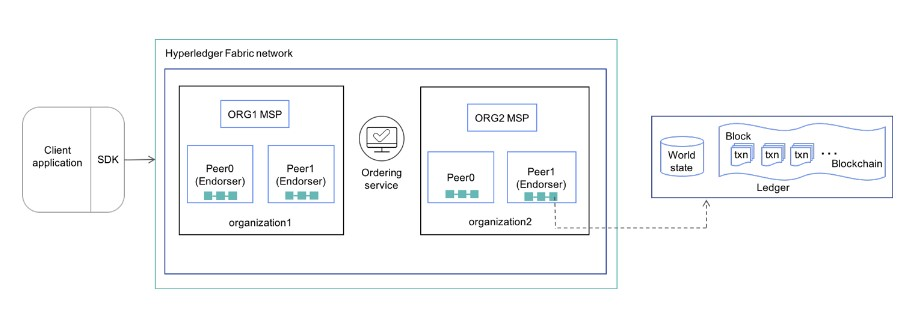
\includegraphics[width=\textwidth]{Images/hlf_components}
\caption{Componentes de Hyperledger Fabric}
\label{fig:hlfcomponents}
\end{figure}


Al igual que otras tecnologías \textit{blockchain}, Hyperledger Fabric cuenta con un \textit{\textbf{ledger}}, utiliza \textbf{contratos inteligentes} y es un sistema mediante el cual los participantes realizan sus \textbf{transacciones}.

Las redes de Hyperledger Fabric son administradas por una colección de \textbf{organizaciones}. Los nodos \textit{\textbf{peer}} son propiedad de estas organizaciones y sus puntos de conexión a la red, por ende, son fundamentales para construir este tipo de red distribuida. 

Al ser una plataforma permisionada, Hyperledger Fabric permite la confidencialidad a través de \textbf{canales}. En estos, los participantes establecen una \textit{sub-red} donde cada miembro tiene visibilidad de un conjunto particular de transacciones. Así, solo aquellos nodos que participan en un canal tienen acceso al contrato inteligente y a los datos transados, preservando la privacidad y confidencialidad de ambos.
Esta es una opción especialmente importante para las redes en las que algunos participantes pueden ser competidores y no desean que cada transacción sea conocida por el resto de la red. 

%Fabric es la primera plataforma DLT que admite \textbf{contratos inteligentes} creados en lenguajes de programación de propósito general como Java, Go y Node.js, en lugar de lenguajes específicos de dominio restringidos (DSL).

\subsection{Ledger}

El \textit{ledger} de Hyperledger Fabric consta de dos componentes: el \textbf{world state} y el \textbf{registro de transacciones}. Cada participante tiene una copia del \textit{ledger} de cada red de Hyperledger Fabric a la que pertenece.

El componente de \textit{world state} describe el estado del \textit{ledger} en un momento determinado y constituye la base de datos del mismo. El componente de registro de transacciones almacena todas las transacciones que dieron como resultado el valor actual del \textit{world state}, o sea, es el historial de actualizaciones del \textit{world state}. En consecuencia, el \textit{ledger} está conformado por la base de datos del \textit{world state} y el historial del registro de transacciones.

\subsection{Contratos inteligentes}

Los desarrolladores de aplicaciones de cada organización pueden crear \textbf{contratos inteligentes }para implementar la lógica de negocio de un proceso comercial compartido por los miembros del consorcio. Los contratos inteligentes se utilizan con el fin de asistir en la generación de \textbf{transacciones}, las cuales pueden ser distribuidas a cada nodo de la red.

Los contratos inteligentes de Hyperledger Fabric se definen dentro del \textbf{\textit{chaincode}}. Se pueden definir múltiples contratos inteligentes en el mismo \textit{chaincode}. Cuando este se despliega en los nodos \textit{peer}, todos los contratos inteligentes dentro del mismo se hacen disponibles para las aplicaciones externas a la \textit{blockchain}. Una aplicación  invoca al contrato inteligente cuando esta necesita interactuar con el \textit{ledger}. 

En la mayoría de los casos, el \textit{chaincode} interactúa sólo con el componente de la base de datos del ledger, el \textbf{\textit{world state}} (consultándolo, por ejemplo) y no con el registro de transacciones.

Los usuarios de Hyperledger Fabric a menudo usan los términos \textbf{contrato inteligente} y \textbf{\textit{chaincode}} indistintamente. En general, un contrato inteligente define la lógica de transacción que controla el ciclo de vida de un objeto contenido en el \textit{world state}; luego, este se empaqueta en un \textit{chaincode} para desplegarse en una red \textit{blockchain}.

\subsection{Consenso}
Las transacciones deben escribirse en el ledger en el orden en que ocurren, aunque puedan ser entre diferentes conjuntos de participantes dentro de la red. Para que esto suceda, se debe establecer el orden de las transacciones y se debe implementar un método encargado de rechazar transacciones incorrectas que se intenten insertar en el ledger por error o maliciosamente.

Los \textit{peers} ejecutan un \textbf{protocolo de consenso} que abarca desde la propuesta y la aprobación de transacciones hasta el orden, la validación y el despliegue de las mismas a través de la red.
En pocas palabras, el \textbf{consenso} se define como la verificación completa de la correctitud de un conjunto de transacciones que componen un bloque [\cite{hlf-doc}].

El consenso está mediado por nodos especiales llamados \textit{\textbf{orderers}}, encargados de ordenar las transacciones. Un conjunto de nodos \textit{orderers} forman un \textbf{\textit{ordering service}}. Además de su rol de ordenar, estos nodos también mantienen la lista de organizaciones que pueden crear canales. Esta lista se conoce como el \textbf{consorcio}.

%Sin embargo, el consenso abarca más que simplemente acordar el orden de las transacciones, y esta diferenciación se destaca en Hyperledger Fabric a través de su papel fundamental en todo el flujo de transacciones, desde la propuesta y el respaldo hasta el pedido, la validación y el compromiso. 

\subsection{Arquitectura \textit{execute-order-validate}.}

Fabric admite el uso de lenguajes de programación estándar en sus contratos inteligentes. Esto gracias a que implementa una arquitectura \textit{execute-order-validate} para el manejo de ejecución de transacciones.

%Para entender por qué es posible añadir $C\sharp$ a la lista de lenguajes soportados por Hyperledger Fabric para programar contratos inteligentes, se dedicará esta sección a explicar dicha arquitectura.

Todos los sistemas de blockchains anteriores a Hyperledger Fabric, permisionados o no, siguen la arquitectura  \textit{order-execute} [\cite{hlf-paper}] para la gestión de transacciones. Esto significa que la red blockchain ordena las transacciones primero, utilizando un protocolo de consenso, y luego los ejecuta en el mismo orden en todos los nodos \textit{peer} secuencialmente.

%La arquitectura \textit{order-execute} es conceptualmente simple y por lo tanto también muy utilizada. Sin embargo, tiene varios inconvenientes cuando se implementa en una blockchain autorizada de uso general.

Un problema importante para una arquitectura \textit{order-execute} son las transacciones no deterministas. Las operaciones que se ejecutan después del consenso deben ser deterministas o el \textit{ledger} distribuido se “bifurca” y viola la premisa básica de una blockchain, la cual garantiza un estado consistente entre todos los nodos \textit{peers}, es decir, todos presenten el mismo estado en sus respectivos \textit{ledger}. Esto generalmente se aborda mediante la programación de \textit{blockchains} en un DSL (ej. Ethereum Solidity), pues son lo suficientemente expresivos para sus aplicaciones pero limitados a una ejecución determinista.

Dichos lenguajes son difíciles de diseñar y requieren generalmente una asimilación de aprendizaje adicional por parte del programador. La redacción de contratos inteligentes en un lenguaje de propósito general (p. ej., Go, Java, C/C++) parece más atractivo y acelera la adopción de soluciones \textit{blockchain}.

%Desafortunadamente, los lenguajes de propósito general plantean muchos problemas para garantizar una ejecución determinista. Incluso si el desarrollador de la aplicación no introduce operaciones obviamente no deterministas, detalles ocultos de implementación pueden tener el mismo efecto devastador (por ejemplo, un
%iterador de mapa no es determinista en Go).

Fabric introduce la arquitectura \textit{order-execute-validate} y no sigue el diseño \textit{order-execute} anteriormente mencionado. La figura \ref{fig:transactionflow} muestra el flujo de una transacción bajo este nuevo modelo.\\[5cm]

\begin{figure}[tbph]
\centering
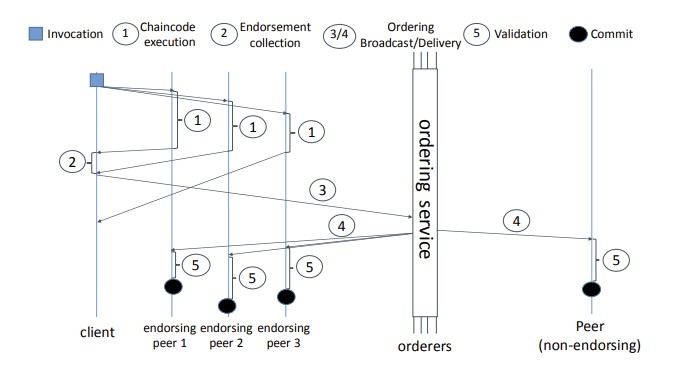
\includegraphics[width=\textwidth]{Images/transaction_flow}
\caption{Flujo de una transacción}
\label{fig:transactionflow}
\end{figure}


Fabric aborda los desafíos de resiliencia, flexibilidad, escalabilidad, rendimiento y confidencialidad que enfrenta el modelo \textit{order-execute} al separar el flujo de transacciones en tres pasos:

\begin{enumerate}
 \item \textbf{ejecutar} una transacción y verificar su correctitud, avalándola.
 \item \textbf{ordenar} transacciones a través de un protocolo de consenso.
   \item \textbf{validar} transacciones contra una política de aprobación específica de la aplicación antes de actualizar el \textit{ledger}.
\end{enumerate}

Este diseño se aparta del paradigma \textit{order-execute} pues Fabric ejecuta transacciones antes de llegar a un acuerdo final sobre su orden. De esta forma se elimina cualquier no determinismo, ya que los resultados inconsistentes se pueden filtrar antes de ordenar.

Al eliminar el no determinismo, Fabric permite el uso de lenguajes de programación estándar en sus contratos inteligentes. 

%Gracias a esta posibilidad, en este trabajo se pretende añadir $C\sharp$ a la lista de lenguajes actualmente soportados.

%\subsection*{Flujo de una transacción}
%El flujo de solicitud de alto nivel de una transacción en una red de Hyperledger Fabric es así:
%
%\begin{enumerate}
%\item El cliente se conecta a una red de Hyperledger Fabric mediante Node.js o Java™ SDK. Usando la API SDK, el cliente crea una transacción y la envía al par que la respalda.
%
%\item El par que respalda verifica la firma del cliente, simula una transacción y envía una firma de respaldo.
%
%\item Si la transacción está endosada, el cliente envía la transacción al servicio de pedidos. De lo contrario, la transacción se cancela.
%
%\item El servicio de pedidos entrega una transacción a los pares. Todos los pares comprometen y aplican la misma secuencia de transacciones y actualizan su estado.
%\end{enumerate}




%Los lenguajes actualmente soportados son Java, Go y Node.js.
%Para entender cómo es posible añadir otro lenguaje para implementar contratos inteligentes, se hará énfasis en la fase de ejecución, donde el chaincode y el nodo peer se comunican. 

%\section{Fase de ejecución}
%
%En la fase de ejecución, los clientes firman y envían la propuesta de transacción a uno o más nodos \textit{peers} para su ejecución.  La propuesta es una solicitud para invocar una función del \textit{chaincode} con ciertos parámetros de entrada, con la intención de leer y/o actualizar el \textit{ledger}. Una aplicación que aprovecha un SDK compatible (Node, Java, Go) utiliza una de las API disponibles para generar una propuesta de transacción.
%
%El SDK sirve como un \textit{shim} para empaquetar la propuesta de transacción en el formato diseñado correctamente (\textit{protocol buffer} sobre gRPC) y toma las credenciales criptográficas del usuario para producir una firma única para esta propuesta de transacción. 



\section{fabric-contract-apis y fabric-chaincode-apis}
En este documento se propone la biblioteca \texttt{fabric-chaincode-csharp} como una herramienta para implementar contratos inteligentes en $ C\sharp $. Por ello, antes de comenzar a describir dicha solución, se hace necesario analizar las ya existentes para otros lenguajes de programación.

Para respaldar el desarrollo de contratos inteligentes (\textit{chaincode}), Hyperledger Fabric ofrece dos APIs por cada lenguaje de programación actualmente soportado (Go, Java y Node.js). Dichas bibliotecas son las llamadas: \texttt{fabric-chaincode-apis }y las \texttt{fabric-contract-api}s.

Las \texttt{fabric-chaincode-apis} son responsables de ejecutar el contrato inteligente, hacerlo accesible para el nodo \textit{peer} y administrar toda la interacción de bajo nivel entre ambos elementos a través de gRPC[\cite{grpc-doc}]. Además, proporcionan la interfaz  \texttt{Chaincode} al contrato inteligente para acceder a los servicios de invocación del \textit{ledger} y el \textit{chaincode}. El módulo chaincode shim, o simplemente shim, constituye el componente principal de las fabric-chaincode-apis.

Las \texttt{fabric-contract-apis} importan las bibliotecas \texttt{fabric-chaincode-apis }y  proveen la interfaz \texttt{Contract}. Esta constituye un punto de entrada de alto nivel que permite abstraer al desarrollador de procedimientos de configuración de la red y concentrarse en implementar la lógica empresarial.

Se hace necesaria 
%
%Ambas bibliotecas propician al desarrollador las herramientas necesarias para implementar contratos inteligentes. En los lenguajes Java y Node.js las fabric-chaincode-apis conforman un módulo dentro de la biblioteca fabric-contract-api. En Go implementa la fabric-chaincode-api 

Actualmente existen tres lenguajes que implementan estas bibliotecas: Go, Java y Javascript/Typescript. Cada una de estas propuestas proveen soluciones distintas a problemas como son: el manejo concurrente de transacciones y la interacción con el peer. A continuación se analizan dichas propuestas.

\subsection{Manejo concurrente de transacciones}
Todas las bibliotecas son capaces de ejecutar múltiples transacciones a la vez (de forma asíncrona). En Go se inicia una \textit{\textbf{rutina go}} para manejar las propuestas de transacciones que vienen del \textit{peer}, mientras que las respuestas de consultas al \textit{ledger} son tratadas en el hilo principal. Por otro lado, en Javascript/Typescript se crea un hilo (\textit{\textbf{stream}}) por cada mensaje recibido, independientemente de su tipo. Lo mismo sucede con la biblioteca de Java.
\subsection{Interacción con el peer} 
Dentro del contexto de una transacción, muchas veces es necesario hacer consultas al \textit{ledger} a través del \textit{peer}. Al ejecutarse las transacciones de forma asíncrona, se requiere organizar este intercambio de mensajes de alguna forma. 

Go crea un diccionario donde a cada transacción se le asocia un \textbf{canal} por donde se envían y reciben mensajes del \textit{peer}. El acceso a dicho diccionario se regula con un objeto \textit{mutex} para asegurar que solo una \textit{rutina go} lo modifique a la vez. Este acercamiento impone como restricción que sólo se puede establecer una comunicación con el peer dentro del contexto de una transacción, es decir, los contratos inteligentes no pueden crear \textit{rutinas go} que interactúen con el peer.

Por otra parte, Javascript/TypeScript y Java implementan la clase \texttt{MsgQueueHandler}. Esta contiene un diccionario donde a cada transacción se le asocia una cola de mensajes. Así, se permite realizar solicitudes concurrentes pues, los mensajes serán añadidos a la cola y enviados uno a uno. Cada vez que se envía una consulta al peer se espera por la respuesta para mandar la próxima.

% un diccionario donde a cada transaccion se le asocia una cola de mensajes. Este acercamiento no impone restricciones al programador pues, aunque existan varios hilos dentro del contrato intelligente la cola garantiza que se envíen en el orden correcto.
%Un contrato inteligente se define dentro de un chaincode. Se pueden definir múltiples contratos inteligentes dentro del mismo chaincode. Cuando se implementa un chaincode, todos los contratos inteligentes dentro de él se ponen a disposición de las aplicaciones.

%La siguiente figura proporciona una descripción general de los componentes principales que están involucrados en la interacción entre el proceso del chaincode y el \textit{peer}.
%
%\begin{figure}[tbph]
%\centering
%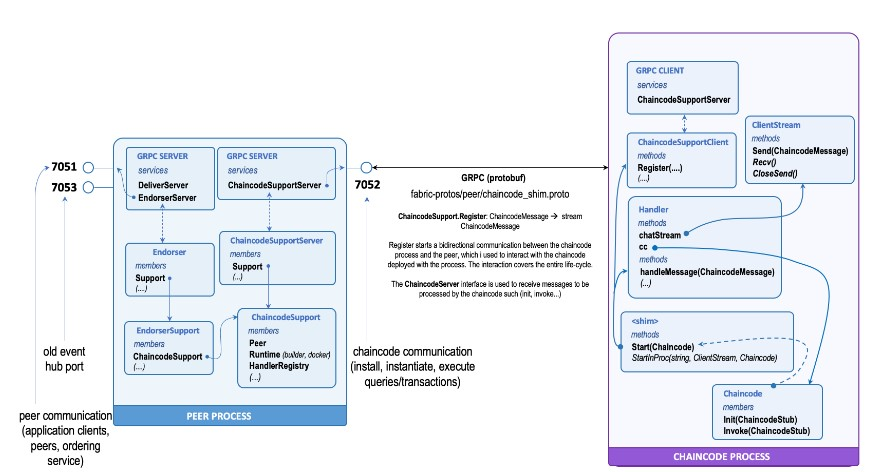
\includegraphics[width=\textwidth]{Images/peer_chaincode_interaction}
%\caption{}
%\label{fig:peerchaincodeinteraction}
%\end{figure}

\section{gRPC y \textit{protocol buffers}}
Como se mencionaba anteriormente, en el \textit{chaincode} se define la lógica de negocio de la aplicación \textit{blockchain} utilizando un lenguaje de programación de propósito general. Los \textit{chaincode} se ejecutan en un entorno desacoplado al resto del nodo \textit{peer}. De esta forma, el \textit{peer} es independiente del lenguaje real en el que se implementa el chaincode. Para cumplir el propósito de este trabajo es necesario implementar un \textit{chaincode} en $ C\sharp$, lenguaje distinto al del nodo peer (Go). En esta sección se explica gRPC  [\cite{grpc-doc}]\footnote{Llamada a Procedimiento Remoto gRPC}, herramienta que permite la comunicación entre ambos elementos. 

En gRPC, una aplicación cliente puede llamar directamente a un método en una aplicación servidor en una máquina diferente como si fuera un objeto local, lo que facilita la creación de aplicaciones y servicios distribuidos que necesitan operar en tiempo real. 

%Como en muchos sistemas RPC, gRPC se basa en la idea de definir un servicio, especificando los métodos que se pueden llamar de forma remota con sus parámetros y tipos de devolución. En el lado del servidor, se implementa una interfaz para manejar las llamadas de los clientes. En el lado del cliente se tiene el \textit{stub}),el cual proporciona los mismos métodos que el servidor.

La diferencia con otros frameworks RPC existentes radica en la capacidad de gRPC de utilizar \textit{protocol buffers} [\cite{protobuf-doc}] como lenguaje de definición de interfaz para la serialización y como formato de intercambio de mensajes, en lugar de JSON/XML.
%
Los \textit{protocol buffers} proporcionan un mecanismo extensible, independiente del idioma y de la plataforma, para serializar datos estructurados de manera compatible con versiones anteriores y posteriores. Se pueden ampliar con nueva información sin invalidar los datos existentes ni requerir que se actualice el código.

\begin{figure}[tbph]
\centering
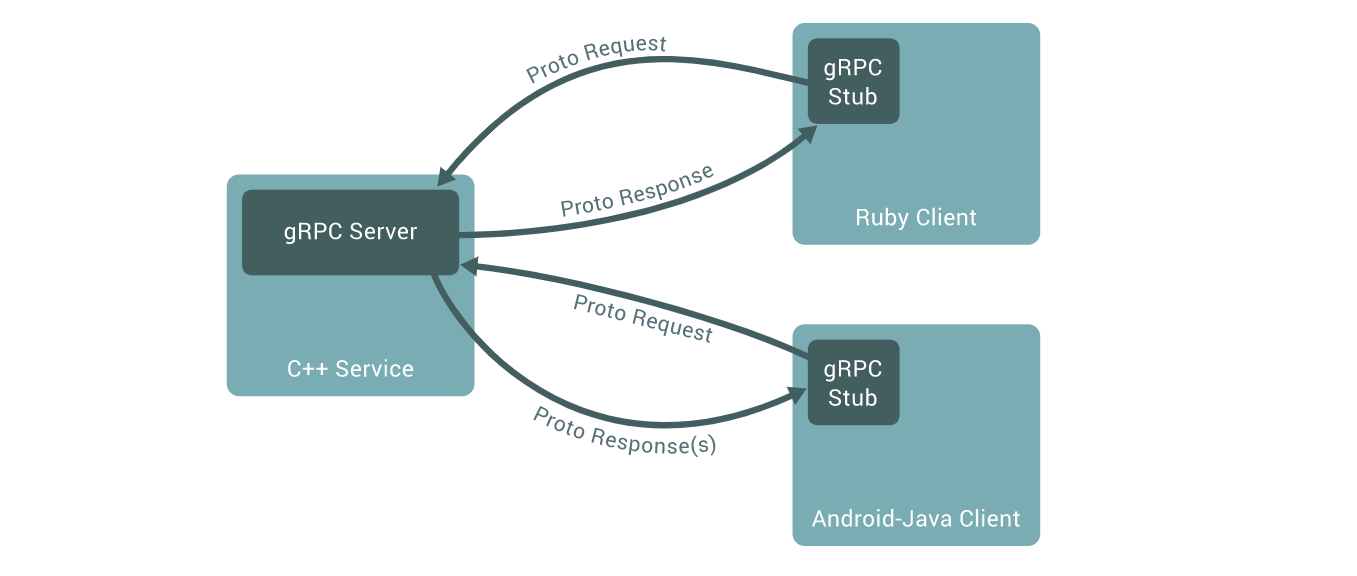
\includegraphics[width=\textwidth]{Images/grpc}
\caption{ Interacción entre cliente y servidor en gRPC.}
\label{fig:grpc}
\end{figure}

Los clientes y servidores de gRPC pueden ejecutarse y comunicarse entre sí en una variedad de entornos y pueden escribirse en cualquiera de los idiomas compatibles con gRPC. La figura \ref{fig:grpc} muestra un ejemplo de servidor gRPC en $ C++ $ con clientes Ruby y Java. En la solución propuesta en este artículo se aprovecha dicha característica para brindar una interfaz de comunicación entre el nodo \textit{peer} y el \textit{chaincode}, escritos en Go y $ C\sharp$ respectivamente.








